% #############################################################################
% This is Chapter 5
% !TEX root = ../main.tex
% #############################################################################
% Change the Name of the Chapter i the following line
\fancychapter{Results}
\cleardoublepage
% The following line allows to ref this chapter
\label{chap:results}

\par The following results are based on solving the optimisation problem \eqref{eq:multi_cost_bern} with the implementation described in section \ref{sec:description_implementation}.
\par Sequential Quadratic Programming \cite{10.1007/978-0-387-35514-6_7} will be the nonlinear programming solver of choice. Simulations were run on a 4 × Intel\textsuperscript{\textcopyright} Core\texttrademark i5-7200U CPU @ 2.50GHz processor.

\par All of the figures flip x and y axis an

\section{No obstacles}
\todo{metion the limits of acceleration of the medusa model}

\par The first problem will be run for both a single Dubin's car and a single Medusa vehicle, with initial and final states decribed in table \ref{tab:firstproblem} and no obstacles.
\begin{table}[h!]
\begin{tabular}{|l|l|l|}
\hline
Variable & Starting Conditions & Final Conditions \\ \hline
$x$ & 0 & 30 \\
$y$ & 0 & 30 \\
$\psi$ & 0 & $\pi/2$ \\
$u$ & 1 & 1 \\
$v$ & 0 & 0 \\
$\omega$ & 0 & 0 \\
\hline
\end{tabular}
\caption{Initial and final conditions for a basic Motion Problem}
\label{tab:firstproblem}
\end{table}

\todo{write the runtimes on the figures}
\par Figure \ref{fig:noobstacleexamples} shows solutions for order 20. Each accompanied by the running cost function that was used. Both models contain control points to describe $x$ and $y$ positions, which is what the blue lines show. The red lines describe the solution of the Initial Value Problem as described in section \ref{sec:ivproblem}

\begin{figure}[h!]
\centering
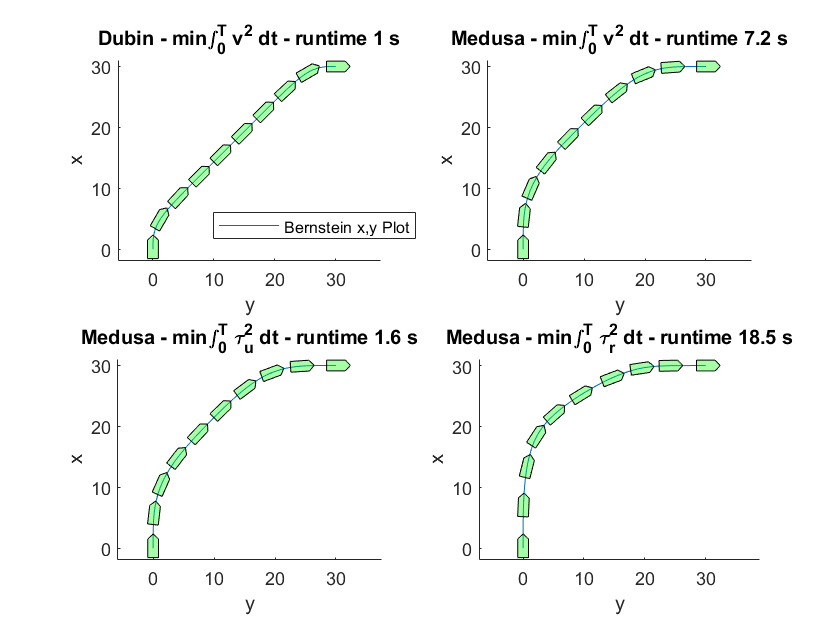
\includegraphics[width=0.8\textwidth]{Images/results/noostaclesfigures.png}
\caption{Solutions of order $N=20$ without obstacles and final time $T=60$}
\label{fig:noobstaclescosts}
\end{figure}

\subsection{Variation of cost with order}
\par We can see how to cost varies with increase of N and how the solution of the \ac{IVP} becomes closer and closer to the plot of $xy$.


\par A noticible difference in the runtime between the 

\par We can see on these solutions 

\section{Obstalces}

\par The following figure shows solutions with circle or polygon obstacles whose collision avoidance algorithms are explained in sections \ref{sec:mindistintveh} and \ref{sec:mindistconvshapes}. Both solutions used The Medusa model.

\begin{figure}[h!]
\centering
\missingfigure[figwidth=6cm]{}
%\includegraphics[width=0.8\textwidth]{Images/results/withobstaclesfigures.png}
\caption{Solutions of order $N=20$ with circular and polygon obstacles}
\label{fig:withobstaclescosts}
\end{figure}

we can see how the iterative min dist to polygon obstacles method adds alot of runtime.



\section{Mulitple Vehicles}

\todo{examples with few vehicles}
\todo{examples with many vehicles}




